\section{Terminology and Background}\label{sec:background} 
This section presents an overview on general concepts necessary to understand this research area, namely Bug Tracking Systems, Machine Learning (algorithms, feature selection methods, evaluation measures, and sampling methods), and Statistical Tests. More specific concepts will be detailed as they are cited in the document.

\subsection{Bug Tracking System (BTS)}

BTS\cite{Lamkanfi:2010} is a software application that keeps the record and tracks information about change requests, bug fixes, and technical support that could occur during the software lifecycle. Usually, while reporting a bug in a BTS, a user is asked to provide information about the bug by filling out a form, typically called bug report form. 

\subsubsection{Bug Report}
Although there is no agreement on the terminology or the amount of information that users must provide to fill a typical bug report (illustrated in Figure \ref{fig:bug-report-example}, the example refers to a bug report extracted from Bugzilla of Eclipse project.), they often describe their needs in popular BTS (e.g., Bugzilla, Jira, and Redmine)\cite{Tian:2012} providing information about at least attributes shown in Table \ref{tab:commom_attributes_bts_form}.  

\begin{table}[!htp] 
  \caption{Commom attributes in a bug report form.}
  \label{tab:commom_attributes_bts_form}
  \centering
  \begin{tabular}{|l|p{6cm}|}
    \hline
    Type & Type of report (e.g., bug, improvement, and new feature)\\
    \hline
    Summary & Short description of report in one line.\\
    \hline
    Description & Long and detailed description of report in many lines of text. It could include source code snippets and stack tracing reports.\\
    \hline
    Severity & Level of severity of report (e.g., blocker, critical, major, minor and trivial).\\
    \hline 
  \end{tabular}
\end{table}

After the user has reported a bug, the development team is in charge of its assessment. The assessment consists of approving or, for some reason (e.g., duplication), not approving the bug. In case of approval, this team may provide complementary information by, for example, assigning a person to be responsible for handling this request or defining a new severity level for the report. Typically, the sequence of steps a bug report goes through is modeled as a state machine. Figure~\ref{fig:life-cycle-of-bug-report} shows an example of such a state machine, with a typical set of states a bug report can hold during its lifecycle in a BTS. Initially, a bug report is in \textit{Unconfirmed} state. The developer team will change the bug report state to \textit{Resolved}, if the bug were not confirmed, or, otherwise, to \textit{New}. When someone was in charge to fixing the bug, the bug report state will be changed to \textit{Assigned} by the developer team. Therefore, in the standard flow, the bug report status will be assigned to resolved (bug fixed), then verified (bug checked), and finally closed. As shown in Figure~\ref{fig:life-cycle-of-bug-report}, others state transitions may occur throughout the bug report lifecycle. All changes occurred in a bug report are stored in a repository, keeping valuable historical information about a particular software.

\begin{figure}[!tp]
  \centering
  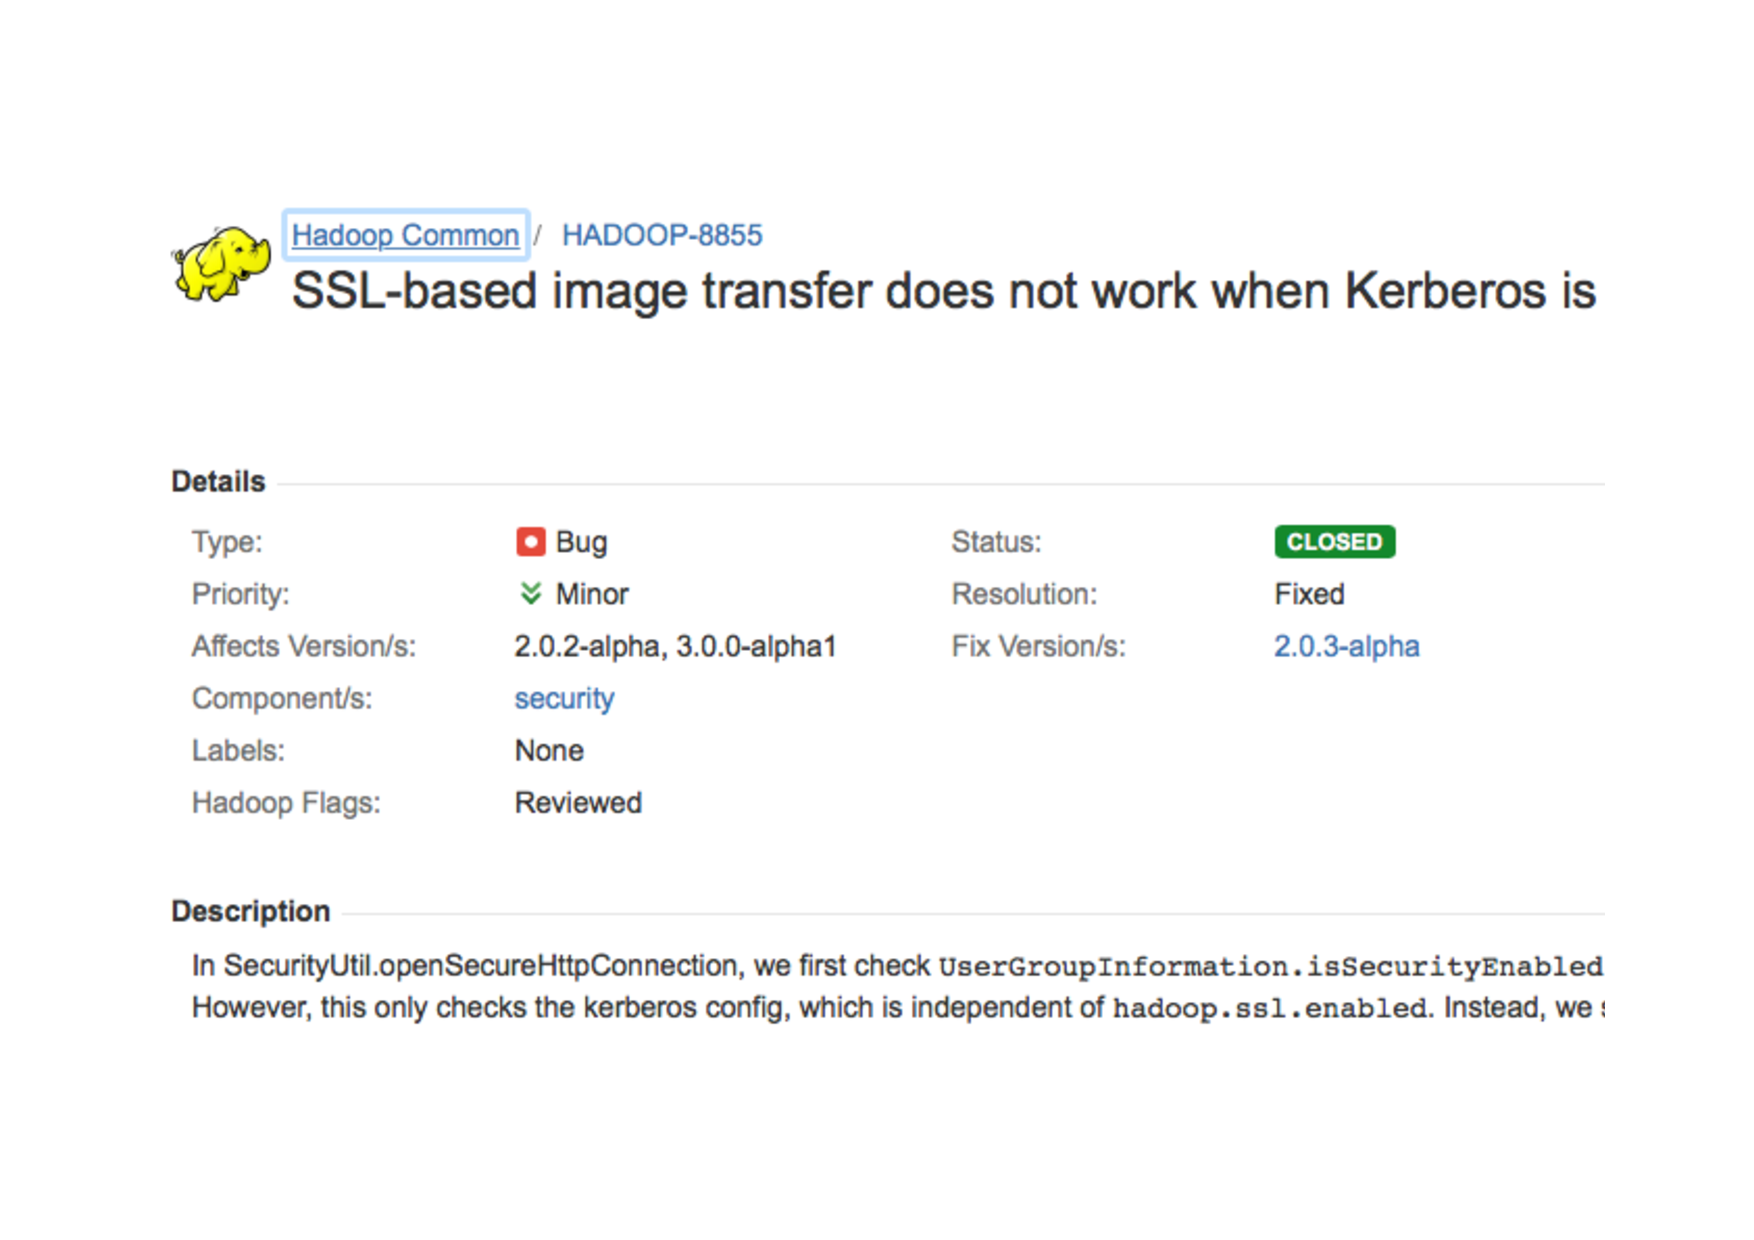
\includegraphics[width=1\textwidth]{figures/bug-report-example.pdf}
  \caption{A typical bug report (\url{https://issues.apache.org/jira/browse/HADOOP-8855}, as of September 2018)} 
  \label{fig:bug-report-example}
\end{figure}

\begin{figure}[!htp]
  \begin{subfigure}{.49\textwidth}
    \centering
    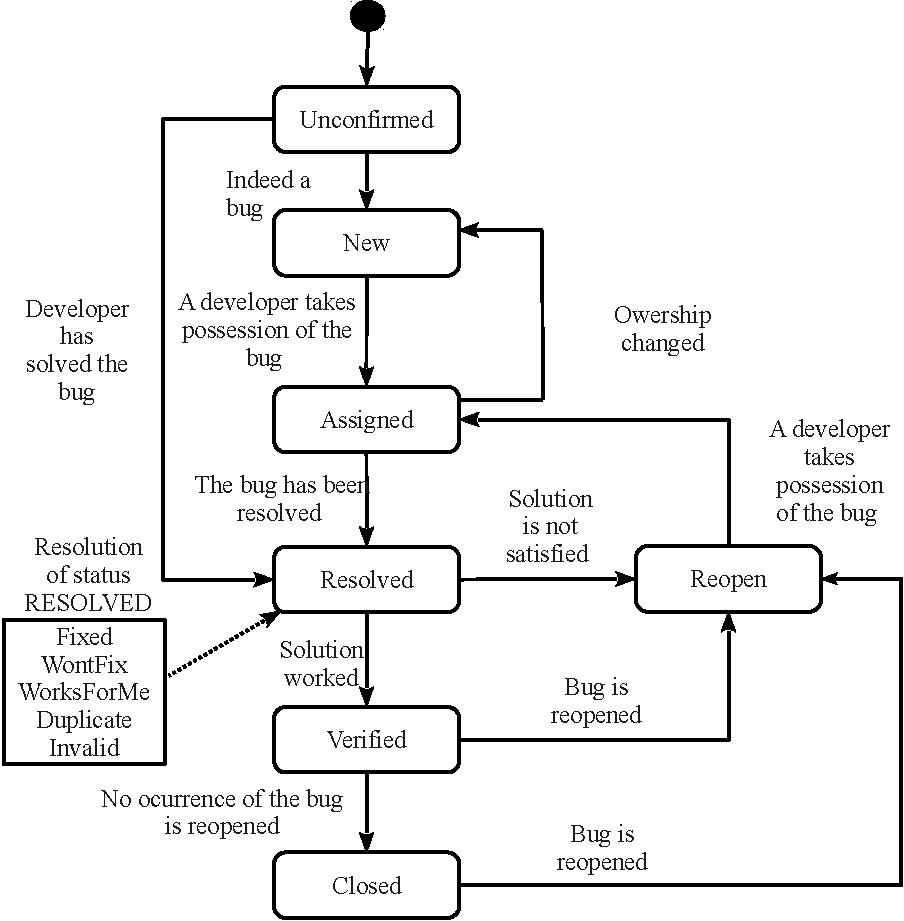
\includegraphics[width=\textwidth]{figures/bug-report-life-cycle.pdf}
    \caption{}
    \label{fig:life-cycle-of-bug-report}
  \end{subfigure}\hfill
  \begin{subfigure}{.40\textwidth}
    \centering
    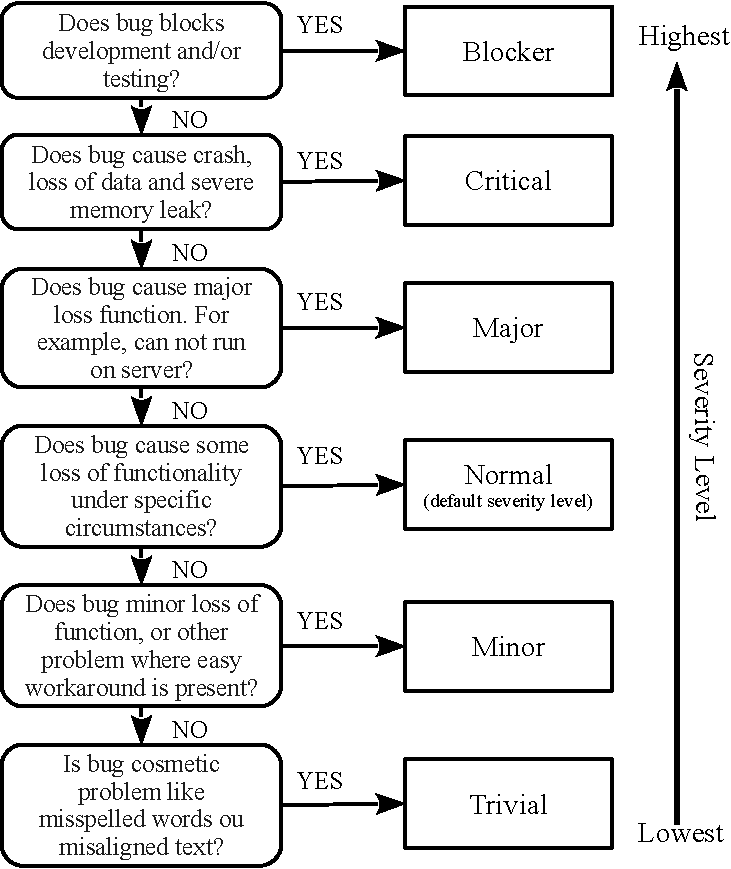
\includegraphics[width=\textwidth]{figures/bug-report-severity-levels.pdf}
    \caption{} 
    \label{fig:bug-report-severity-level-guideline}
  \end{subfigure}
  \caption{(a) The bug report lifecycle according to Zhang et al.\cite{Zhang:2015}. (b) Bugzilla guideline for bug report severity level assignment (\url{https://www.bugzilla.org}, as of \today).}
  \label{fig:bug-report-life-cycle-and-severity-level-guideline}
\end{figure}

Both users and development team members can define or redefine the severity level for a bug during the lifecycle. Figure \ref{fig:bug-report-severity-level-guideline} illustrates Bugzilla guidelines for assigning bug severity level. The Figure shows that such choices should be based on an affirmative answer to a question which characterizes a severity level appropriately. Also, the Figure indicates that \textit{Trivial} and \textit{Blocker} are lower and higher respectively.

To predict severity level, researchers sometimes aggregate these levels in severe (blocker, critical, and major) and non-severe (normal, minor and trivial) to work with a coarse-grained classification problem. Furthermore, some of them ignore the default severity level (often ``normal") because they consider this level as a choice made by users when they are not sure about the correct severity level. Other studies choose to predict a bug report severity level as \textit{blocking} or \textit{non-blocking} bug. A blocking bug is one that prevents other bugs to be fixed\cite{Valdivia:2014}. 

\subsection{Machine Learning}
Machine Learning (ML)\cite{Flach:2012} is an application of Artificial Intelligence (AI) that provides systems the ability to learn and improve from experience without being explicitly programmed. There are two types of ML algorithms: predictive (or supervised) and descriptive (or unsupervised). A predictive algorithm builds a model based on historical training data and uses this model to predict, from the values of input attributes, an output label (class attribute) for a new sample. A predictive task is called classification when the label value is discrete, or regression when the label value is continuous. 

On the other hand, a descriptive algorithm explores or describes a dataset. There is not an output label associated with a sample. Data clustering and pattern discovery are two examples of descriptive tasks. Bug report severity prediction is considered a classification problem; therefore, more detailing of descriptive algorithms are outside the scope of this paper.

\subsubsection{ML algorithms}
A ML algorithm works over a dataset, which contains many samples or instances $x_{i}$, where $i = \{1..n\}$. Each instance is composed of $\{x_{i1}, x_{i2},...,x_{id}\}$ input attributes or independent variables, where $d = \{1..m\}$, and one output attribute or dependent variable, $x_{i(m+1)}$.  Input attributes are commonly named features or feature vector, and output attribute as commonly named class or category. The most traditional ML classification algorithms are k-Nearest Neighbors, Näive Bayes, Decision Tree, Neural Networks, Random Forest and Support Vector Machine. In practice, they can be applied for both classification and regression tasks. However, this mapping review regards them only in the classification scenario. Next, a brief description of each one is presented\cite{Marsland:2014}:

\begin{itemize}
  \item \textbf{k-Nearest Neighbors} (k-NN) process the available instances (or neighbors) in a dataset and classifies a new instance based on its similarity measure to the k-nearest neighbors. Usually, k-NN algorithms utilize a Euclidean distance to quantify the proximity of neighbors. To calculate this distance, each feature vector of each instance in a dataset should represent a point of an n-dimensional space.
  
  \item \textbf{Näive Bayes} (NB) decides to which class an instance belongs based on the Bayesian Theorem of conditional probability. The probabilities of an instance belonging to each of the $C_{k}$ classes given the instance $x$ is $P(C_{k}|x )$. Näive Bayes classifiers assume that given the class variable, the value of a particular feature is independent of the value of any other feature.
  
  \item \textbf{Decision Tree} consists of a collection of internal nodes and leaf nodes in a tree, organized in a hierarchical model.  Each internal node represents a feature, and each leaf node corresponds to a class label. The decision tree classifiers organize a series of test questions and conditions in a tree structure.  A decision tree represents the model capable of guiding the decision making on the determination of the class to which an individual belongs.
  
  \item \textbf{Neural Network} is a learning algorithm that is inspired by the structure and functional aspects of biological neural networks\cite{Haykin:1998}. It structured as a network of units called neurons, with weighted, directed connections. Neural network models have been demonstrated to be capable of achieving remarkable performance in document classification\cite{Zhou:2012}.  \rem{Figure \ref{fig:artificial-neuron} presents an artificial neuron model that contains a set of weighted inputs ($w_i$), which corresponds to the synapses; an adder function ($\sum$) that sums the inputs signals; and an activation function ($f(.)$) that decides whether the neuron fires for the current inputs to generate the output value ($y_{o})$. Independent features of each instance represent neuron dendrites.}
  \rem{
  \begin{figure}[h!]
    \centering
    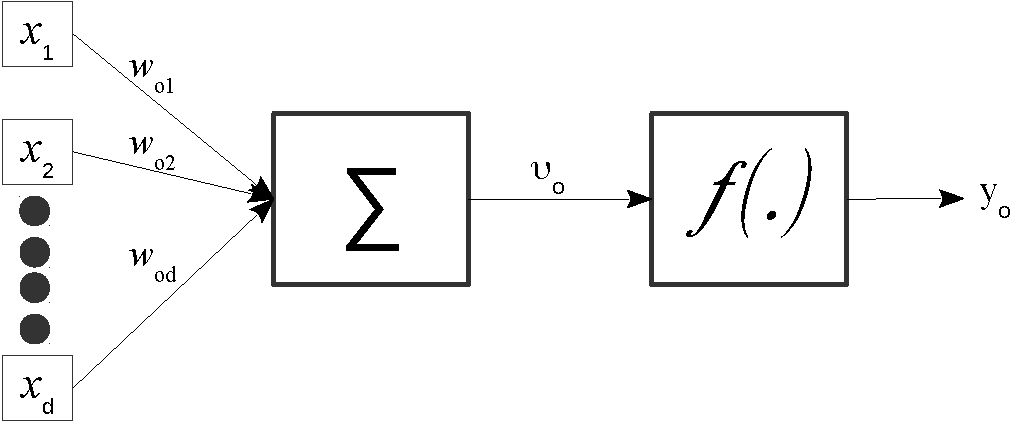
\includegraphics[width=0.5\textwidth]{figures/artificial-neuron.pdf}
    \caption{A artificial neuron model based on Marsland \cite{Marsland:2014}.}
    \label{fig:artificial-neuron}
  \end{figure}
  }
  \item \textbf{Support Vector Machine(SVM)}\rem{represents each feature vector of each instance as a point in an n-dimensional space. The algorithm divides every point belonging to a category in a particular space. Each space is separated by a gap that is as wide as possible\cite{Marsland:2014}. \rem{This space between these two regions delimits the margin between classes.}In Figure \ref{fig:support-vector-machine}, for example, SVM will search for support vectors which are instances located at the edge of an area in space. Such vectors define boundaries between one of these class instances (e.g., the crosses) and instances from another class (e.g., the circles).  \rem{Each region contains instances belonging to the same class\cite{Williams:2011}}. New instances are then mapped into that same space and predicted to belong to a category based on which side they are.}\edit{Each  feature vector of each instance is a point in an n-dimensional space.  SVM learns in this space an optimal way to separate the training instances according to their class labels. The output of this algorithm is a hyperplane, which maximizes the separation among feature vectors of instances of different classes. Given a new instance, SVM assigns a label based on which subspace  its feature vector belongs to~\cite{Tian:2016}.}
\rem{
  \begin{figure}[h!]
    \centering
    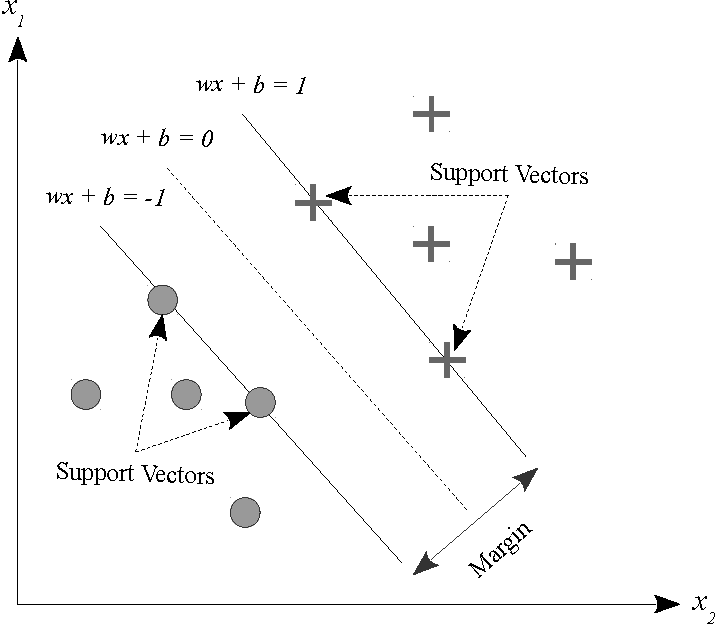
\includegraphics[width=0.4\textwidth]{figures/support-vector-machine.pdf}
    \caption{A SVM model example.}
    \label{fig:support-vector-machine}
  \end{figure}
}
  \item \textbf{Random Forest}\cite{Breiman:2001} relies on two core principles: (i) the creation of hundreds of decision trees and their combination into a single model; and (ii) the final decision is based on the ruling of the majority of the forming trees. 
\end{itemize}

\subsubsection{Feature Selection Methods}
Feature selection is the process of choosing a subset of features that better contribute to the accuracy of a predictive model. Three typical feature selection methods are described next\cite{Zheng:2004}:

\begin{itemize}
  \item \textbf{Information Gain (IG)}:  this method measures the number of bits of information obtained for category prediction by knowing the presence or absence of a feature in a dataset.
  \item \textbf{Chi-square (CHI)}: this method measures the lack of independence between a feature $f$ and category $c_i$ and can be compared to the chi-square distribution with one degree of freedom.
  \item \textbf{Correlation Coefficient (CC)}:  this method defines the correlation coefficient of feature $f$ with a category $c_i$.    
\end{itemize}

\subsubsection{Evaluation measures}
Accuracy, precision, recall, and F-measure are four measures commonly used to evaluate the performance of prediction models\cite{Feldman:2006}. The computation of the values of these measures are based on a \textit{confusion matrix}\cite{Williams:2011}, which represents the number of true/false positives, and the number of true/false negatives for each instance class value when making a prediction. Each measure is described next \cite{Japkowicz:2011}: 

\begin{itemize}
  \item \textbf{Accuracy} is the percentage of correctly classified observations among all observations:
  
  \begin{equation}
  Accuracy = \frac{TP+TN}{P+N}
  \end{equation}
  
  where P is the total of positive class instances, N is the total of negative class instances, TP is the number of true positives, and TN is the number of true negatives.
  
  \item \textbf{Precision} is the percentage of correctly classified observations among all observations that were assigned to the class by the classifier. It can be viewed as a measure of classifier exactness. A low precision can also indicate a large number of false positives. More formally recall is defined as:
  
  \begin{equation}
  Precision = \frac{TP}{TP+FP}
  \end{equation}
  
  where TP is the number of true positives, and FP is the number of false positives.
  
  \item \textbf{Recall} of a classification method can be defined as the percentage of correctly classified observations among all observations belonging to that class. It can be viewed as a measure of a classifiers completeness. A low recall indicates many false negatives in testing classification step. More formally recall is defined as: 
  
  \begin{equation}
  Recall = \frac{TP}{TP+FN}
  \end{equation}
  
  where TP is the number of true positives, and FN is the number of false negatives.
  
  \item \textbf{F-measure} is a harmonic mean of the precision and recall\cite{Feldman:2006}. F-measure can be calculated as:
  
  \begin{equation}
  \textit{F-measure} = \frac{2 \times (precision \times recall)}{(precision + recall)}
  \end{equation}
  
\end{itemize}

Receiving Operating Characteristics (ROC) is an alternative measure to evaluate binary classifiers. A ROC curve\cite{Japkowicz:2011} is a bidimensional chart, where the X-axis represents false positives, and the Y-axis represents true positives. The Area Under ROC Curve (AUC), ranging between 0 and 1, is used to assess the performance of ML algorithms. An algorithm outperforms another one if its AUC value is closer to 1. 

\subsubsection{Sampling methods}
The evaluation of the supervised method effectiveness is mainly based on two datasets with labeled samples, one for training the predictive model and the other for testing this model. Assessing performance of a predictive model using the same dataset for training and testing is not recommend and may yield misleading optimistic estimations\cite{Japkowicz:2011}. In order to obtain more reliable predictive estimates, resampling methods can be used to split the entire dataset into a training dataset and a testing dataset. Such methods according to  Facelli et al. \cite{Facelli:2015} include: 
\begin{itemize} 
  \item \textbf{Holdout} splits a dataset into a ratio of \textit{p} for training and $(1 - p)$ for testing. 
  \item \textbf{Cross-Validation (CV)} divides a dataset into $k$ folds. In each iteration, it saves a different fold for testing and uses all the others for training. 
  \item \textbf{Bootstrap} generates \textit{r} training subsets from the original dataset. It randomly samples instances with replacement from this set. Unselected cases make up the test subset. The result is the average performance observed for each test subset.
\end{itemize}

\subsubsection{Statistical tests}
\edit{Many scenarios require running several ML algorithms to chose the best predictive model. Even though the performance of these algorithms may be shown to be different on specific datasets, it needs to be confirmed whether the observed differences are statistically significant and not merely coincidental\cite{Japkowicz:2011}. In this situation, conducting statistical tests is a recommended practice for reliable comparison between predictive models under investigation\cite{Facelli:2015}. A brief description of four common statistical tests is provided:}

\begin{itemize}
  \item \textbf{T-Test}\cite{Japkowicz:2011} is a parametric statistical hypothesis test that can be used to assess whether the means of two groups are statistically different from each other.
  \item \textbf{Wilcoxon signed-rank test}\cite{Wilcoxon:1992} is a non-parametric statistical hypothesis test that can be used to determine whether two dependent samples, selected from the population, have the same distribution. 
  \item \textbf{Proportion test}\cite{Lewis:2013} is a parametric statistical hypothesis test that can be used to assess whether or not a sample from a population represents the true proportion of the entire population. 
  \item \textbf{Shapiro Wilk test}\cite{Lewis:2013} is a parametric statistical hypothesis test that can be used to test whether a sample $x_1, ..., x_n$ came from a normal distribution of the population.
\end{itemize}


\subsection{Text Mining}
The common ML algorithms cannot directly process unstructured text (e.g., \textit{summary} and \textit{description} fields from bug report form). Therefore, during a preprocessing step, these unstructured text fields are converted into more manageable representations. Typically, the content of these fields is represented by feature vectors, points of an n-dimensional space. Text mining is the process of converting unstructured text into a structure suited to analysis\cite{Feldman:2006}. It is composed of three primary activities\cite{Williams:2011}:

\begin{itemize}
  \item \textbf{Tokenization} is the action to parsing a character stream into a sequence of tokens by splitting the stream at delimiters. A token is a block of text or a string of characters (without delimiters such as spaces and punctuation), which is a useful portion of the unstructured data. 
  \item \textbf{Stop words removal} eliminates commonly used words that do not provide relevant information to a particular context, including prepositions, conjunctions, articles, common verbs, nouns, pronouns, adverbs, and adjectives. 
  \item \textbf{Stemming} is the process of reducing or normalizing inflected (or sometimes derived) words to their word stem, base form—generally a written word form (e.g., ``working” and ``worked" into ``work").
\end{itemize}

Two of the most traditional ways of representing a document relies on the use of a bag of words (unigrams) or a bag of bigrams (when two terms appear consecutively, one after the other)\cite{Feldman:2006}. In this approach all terms represent features, and thus the dimension of the feature space is equal to the number of different terms in all documents (bug reports). Methods for assigning weights to features may vary. The simplest one is to assign binary values representing the presence or absence of the term in each text. Term Frequency (TF), another type of quantification scheme, considers the number of times in which the term appears in each document. Term Frequency-Inverse Document Frequency (TD-IDF), a more complex type of scheme,  takes into account the frequencies of the term in each document, and in the whole collection.  The importance of a term in this scheme is proportional to its frequency in the document and inversely proportional to the frequency of the term in the collection. 